\documentclass[12pt]{article}
\usepackage{pdfpages}
\usepackage{eso-pic}
\usepackage{hyperref,url}
\usepackage{graphicx}
\graphicspath{{images/}}
\newcommand\tab[1][1cm]{\hspace*{#1}}

\begin{document}
\begin{titlepage}

%----------------------------------------------------------------------------------------
% TITLE PAGE INFORMATION
%----------------------------------------------------------------------------------------
\begin{center} % Center everything on the page

%----------------------------------------------------------------------------------------
% HEADING SECTIONS
%----------------------------------------------------------------------------------------
\textsc{\large Facultatea Calculatoare, Informatica si Microelectronica}\\[0.5cm]
\textsc{\large Universitatea Tehnica a Moldovei}\\[1.2cm] % Name of your university/college
\vspace{25 mm}

\textsc{\Large Medii Interactive de Dezvoltare a Produselor Soft}\\[0.5cm] % Major heading such as course name
\textsc{\large Lucrarea de laborator\#2}\\[0.5cm] % Minor heading such as course title
%\textsc{\large Laboratory work}\\[0.5cm] % Minor heading such as course title

\newcommand{\HRule}{\rule{\linewidth}{0.5mm}} % Defines a new command for the horizontal lines, change thickness here

%----------------------------------------------------------------------------------------
% TITLE SECTION
%----------------------------------------------------------------------------------------
\vspace{10 mm}
\HRule \\[0.4cm]
{ \LARGE \bfseries Realizarea unui simplu GUI Calculator  }\\[0.4cm] % Title of your document
\HRule \\[1.5cm]

%----------------------------------------------------------------------------------------
% AUTHOR SECTION
%----------------------------------------------------------------------------------------
\vspace{30mm}

\begin{minipage}{0.4\textwidth}
\begin{flushleft} \large
\emph{Autor:}\\
		Ernest \textsc{Bitca}
		\end{flushleft}
		\end{minipage}
		~
		\begin{minipage}{0.4\textwidth}
		\begin{flushright} \large
		\emph{lector asistent:} \\
			Irina \textsc{Cojanu} \\ % Supervisor's Name 
			\emph{lector superior:} \\
				Radu \textsc{Melnic} % Supervisor's Name
				\end{flushright}
				\end{minipage}\\[4cm]

				\vspace{5 mm}
				% If you don't want a supervisor, uncomment the two lines below and remove the section above
				%\Large \emph{Author:}\\
					%John \textsc{Smith}\\[3cm] % Your name

					%----------------------------------------------------------------------------------------
					% DATE SECTION
					%----------------------------------------------------------------------------------------

					%{\large \today}\\[3cm] % Date, change the \today to a set date if you want to be precise

					%----------------------------------------------------------------------------------------
					% LOGO SECTION
					%----------------------------------------------------------------------------------------

					%\includegraphics{red}\\[0.5cm] % Include a department/university logo - this will require the graphicx package

					%----------------------------------------------------------------------------------------

					\vfill % Fill the rest of the page with whitespace
					\end{center}

					\end{titlepage}


\cleardoublepage

\section*{Lucrarea de laborator \#5}
\phantomsection

\section{Obiectivele lucrarii}

Crearea unei aplicatii complexe in echipa.
~\\
Divizarea sarcinilor pe membrii echipei.

\section{Scopul lucrarii de laborator}

Lucrul in echipa.
~\\
Aplicarea tehnicilor, limbajelor de programare si 
IDE-uri studiate in laboratoarele precedente.

\section{Mersul lucrarii de laborator}

\tab In lucrarea de laborator s-a creat jocul \textbf{"Corewar"}.
Insusi jocul consta in crearea unor \textbf{jucatori} care reprezinta niste \textbf{procese} (programe).
Procesele date sunt incarcate pe un sector de memorie (arena unde vor lupta jucatorii.)
Scopul principal a jucatorilor este se lupte intre ei si sa ramina in viata.
Fiecare jucator este scris intr-un \textbf{pseudo limbaj de programare}, prin urmare ei necesita sa fie compilati
(setul de instructiuni este prezent in fisierul extern).
~\\
\tab Pentru a compila jucatorii s-a creat un \textbf{"compilator"} care va transla instructiunele (Fig 1) intr-un cod care va fi
 perceput de \textbf{"masina virtuala"} (Fig 2).

\begin{center}
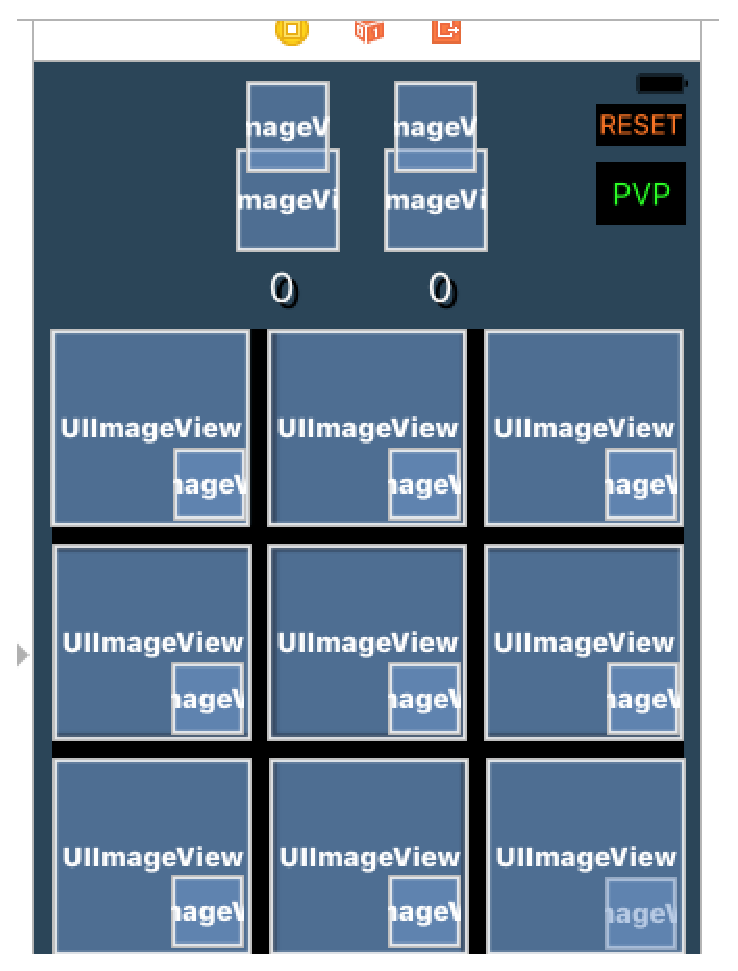
\includegraphics[width=6cm, height=4.8cm]{1.eps}
~\\
Fig 1.
\end{center}
\clearpage

\begin{center}
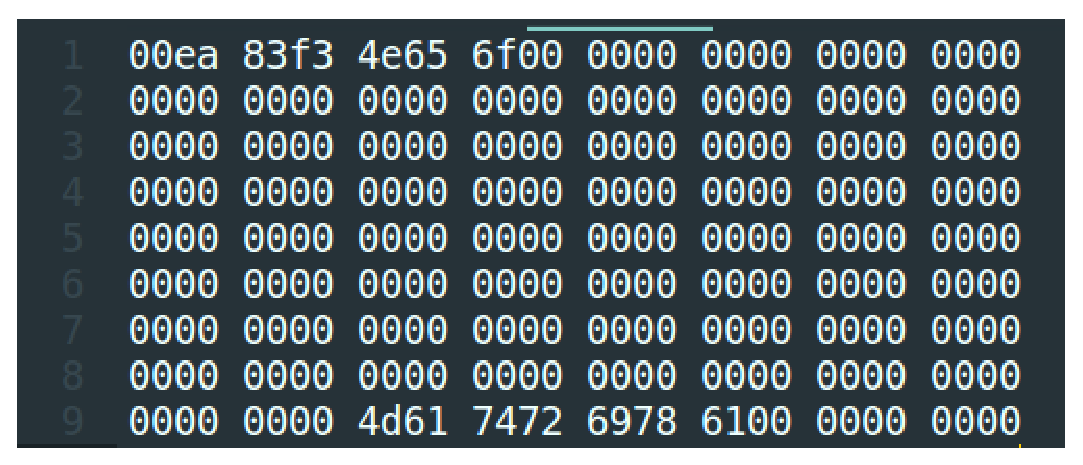
\includegraphics[width=9cm, height=4.2cm]{10.eps}
~\\
Fig 2.
\end{center}

\tab Pentru a compila jucatorul trebuie sa avem un fisier cu extensia \textbf{.s}. In caz contrar vom primi
eroare la compilare. Totodata la compilare se indica rindul in care este prezenta eroarea. Fisierul compilat
se pastreaza sub format \textbf{.cor} (Fig3).


\begin{center}
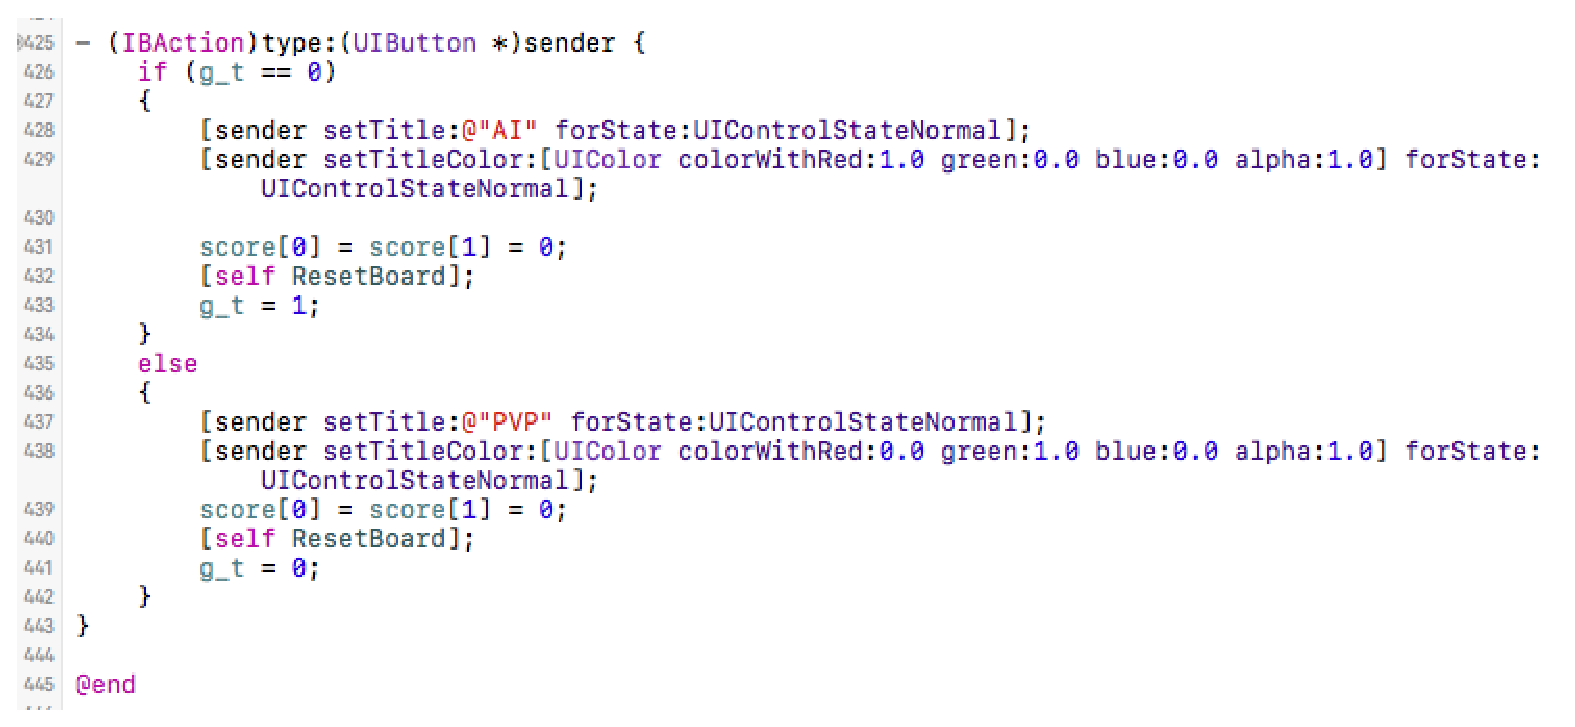
\includegraphics[width=5.9cm, height=4.5cm]{3.eps}
~\\
Fig 3.
\end{center}

Fiecare jucator are numele sau si totodata un comentariu care este indicat la inceputul programului.
Exemplu de pornire a compilatorului (Fig 4).

\begin{center}
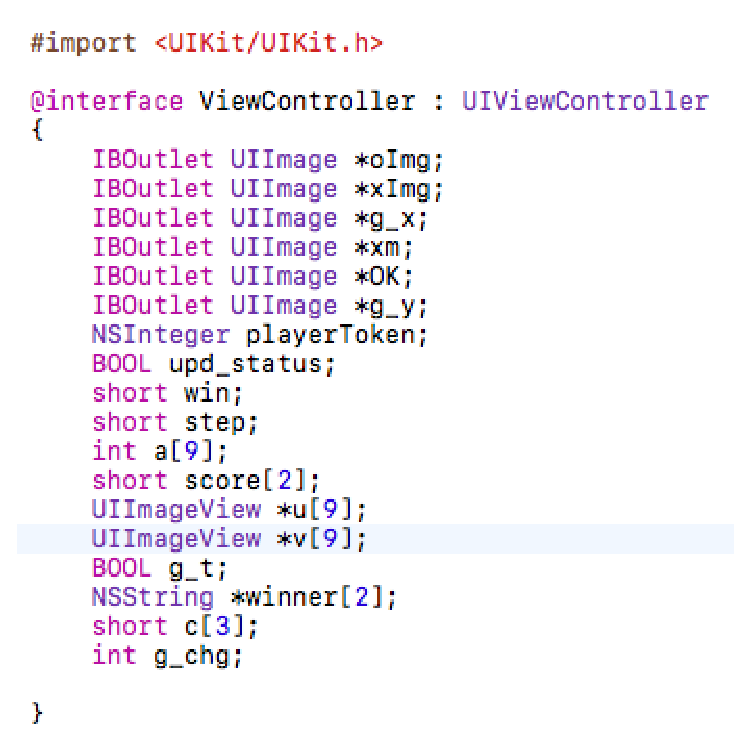
\includegraphics[width=9.5cm, height=3.5cm]{2.eps}
~\\
Fig 4.
\end{center}
\clearpage


\textbf{Secvente de cod}(Fig 5).

\begin{center}
~\\
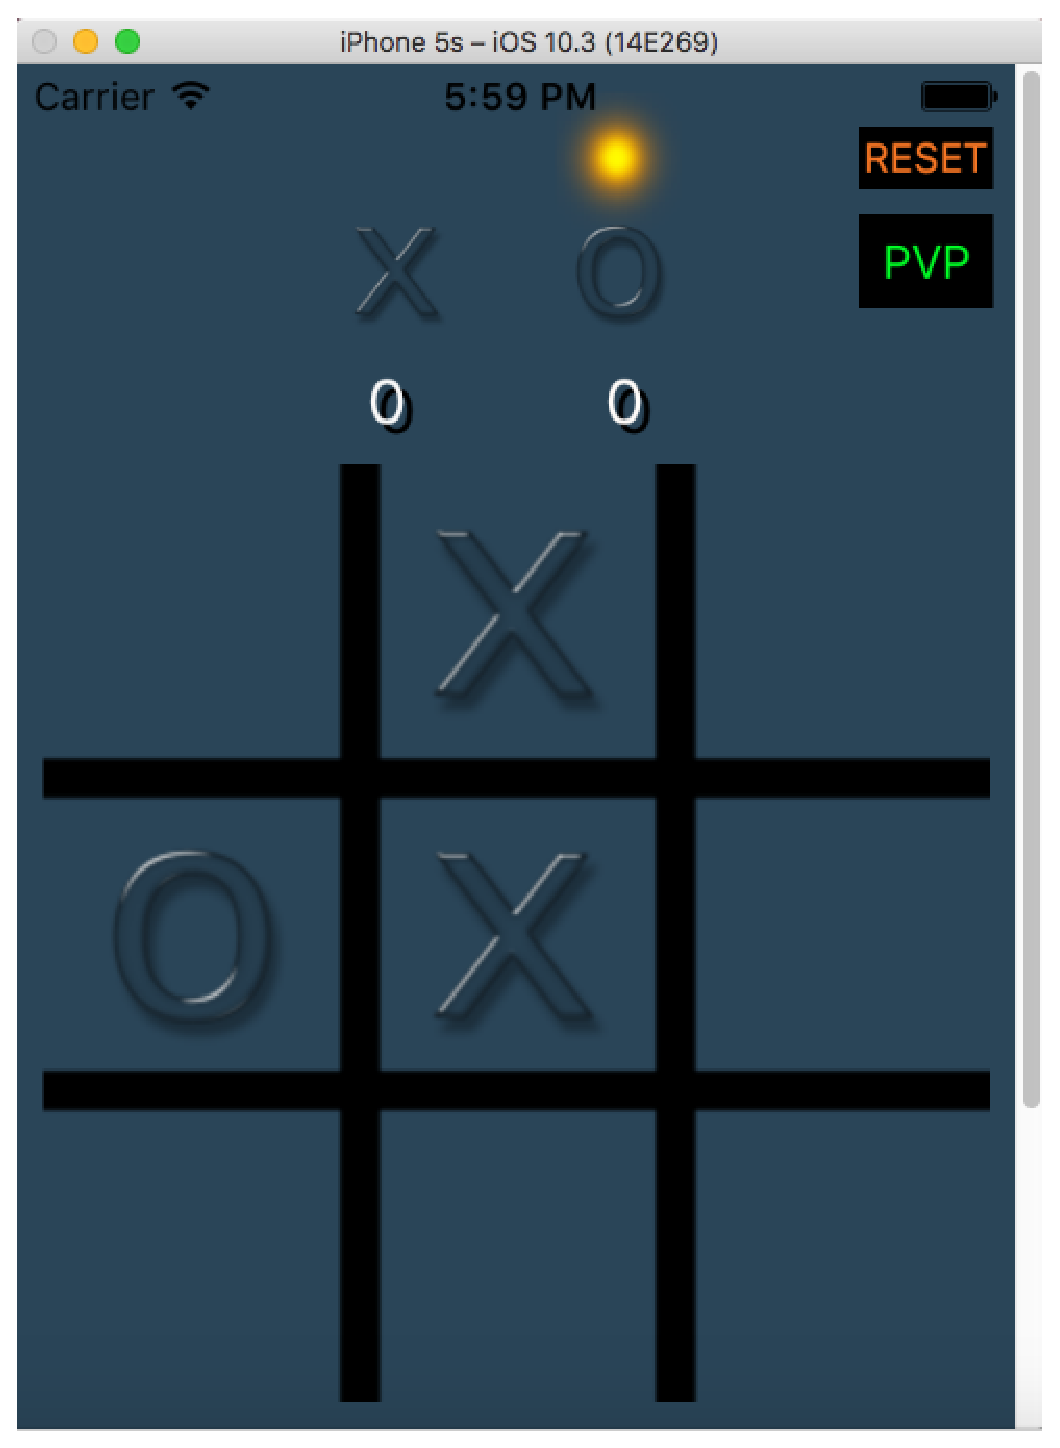
\includegraphics[width=7.3cm, height=8.5cm]{5.eps}
~\\
Fig 5
\end{center}

\section{Regulile jocului}
Fiecare jucator este scris in limbajul asm modificat(RedCode) care prin Compilator se transforma in bytecode.
Codul la fiecare jucator este incarcat in memoria masinei virtuale,care este apoi executat consecutiv.Scopul jocului este de a ramine in viata, pentru asta fiecare jucator trebuie sa execute instructiunea live cu nr lui.Pe linga aceasta instructiune sunt prezente si multe altele: operatiile aritmetice, de incarcare datelor in registri, de accesare si modificare a memoriei ,de creare a proceselor noi.Datorita faptului ca memoria este partajata de toti jucatori, ele pot influenta portiunea de cod a altor jucatori si astfel sa le dauneze, sau chiar sa le "omoare".

\clearpage
\section{Screenshoturi}
\begin{center}
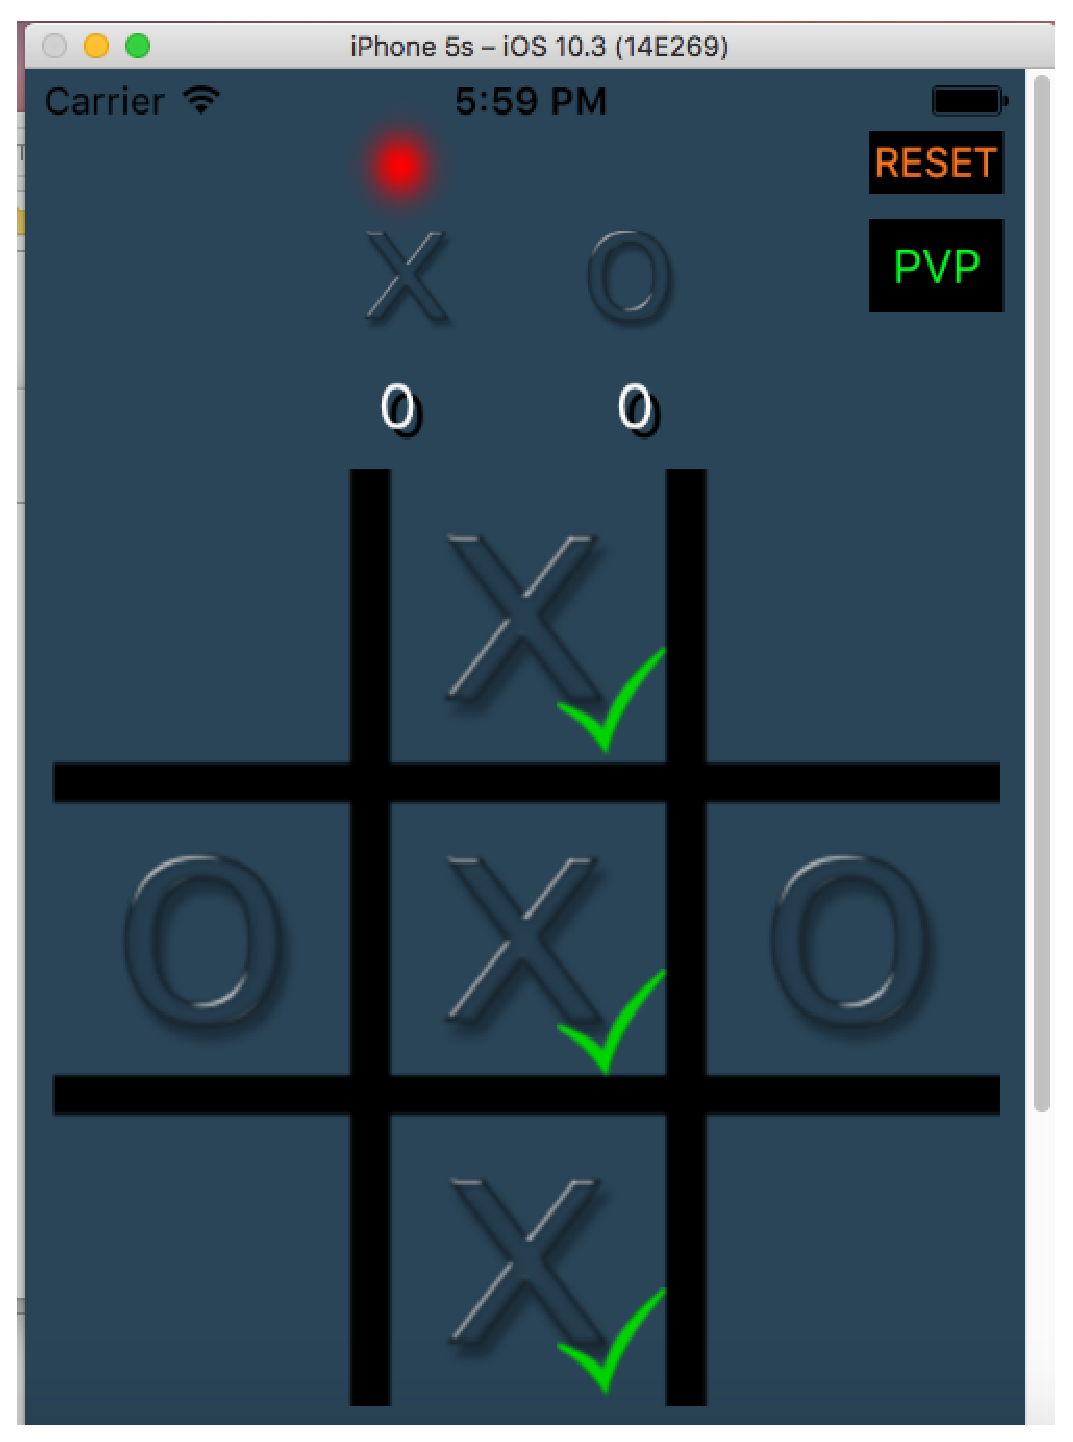
\includegraphics[width=14cm, height=8.5cm]{7.eps}
\end{center}

\begin{center}
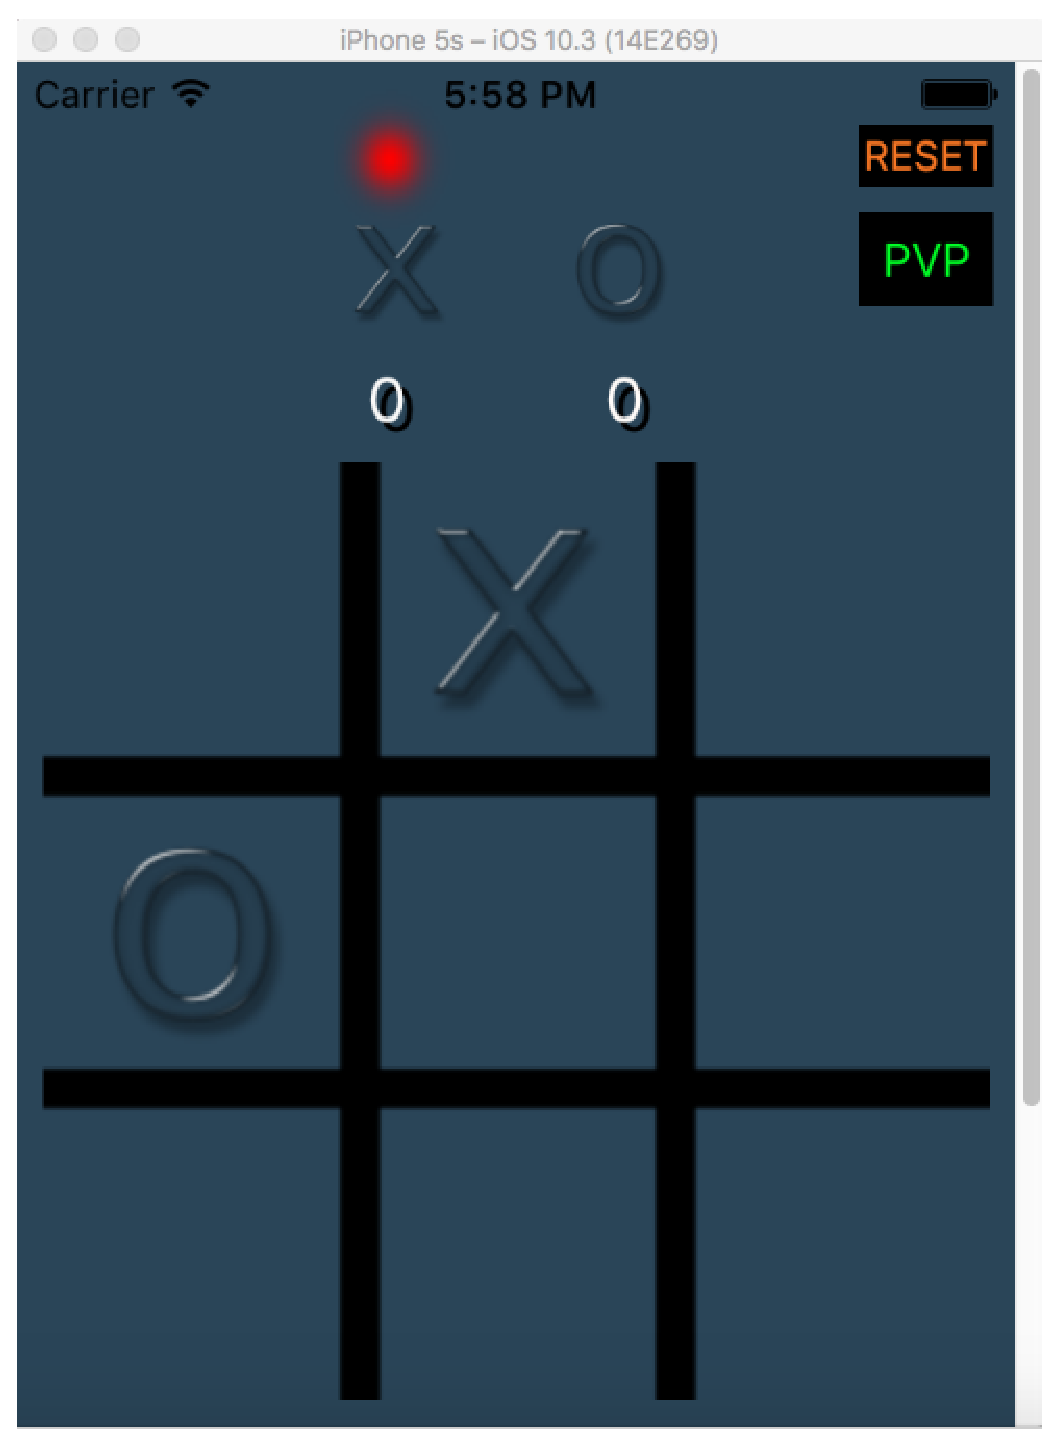
\includegraphics[width=14cm, height=7.5cm]{4.eps}
\end{center}

\section*{Repartizarea lucrului}
\phantomsection

Compilator - Bitca Ernest
~\\
Masina virtuala - Crivenco Vladislav, Lascu Mihai
~\\
Vizualizare - Bitca Ernest

\section*{Concluzie}
\phantomsection

\tab In lucrarea data s-a creat o joaca pentru programatori. A fost impartit proiectul in mai multe parti si fiecare membru
al echipei era responsabil de partea lui. Pentru dezvoltare s-a folosit ca IDE \textbf{Code Blocks}. Pentru afisarea memoriei s-a
folosit biblioteca grafica din C++. Pe parcursul lucrarii s-a studiat conceptul de masina virtuala, s-a lucrat mult cu parsingul si
s-au imbunatatit calitatile de lucru in grup. In echipa se pot efectua proiecte complexe, creste viteza de lucru si totodata scade numarul
de erori, deoarece toti se ajuta reciproc. In concluzie putem spune ca este foarte important de lucrat in echipe si de impartit taskurile 
rational si efectiv intre membri.

\cleardoublepage

\newpage
\section*{Concluzii}
\phantomsection

\tab In lucrarea data s-a creat o aplicatie mobila pe \textbf{IOS}.
Insusi aplicatia reprezinta o joaca (Tic-Tac-Toe). Joaca suporta doua regimuri.
Dupa fiecare joc cistigat - jucatorii acumuleaza puncte. Pe parcursul lucrarii s-a utilizat
masina virtuala pentru a virtualiza sistemul de operare Mac OS Sierra. Ca IDE s-a folosit
\textbf{XCode 8.3.1}. Au fost adaugate butoane de resetare a jocului, totodata dupa fiecare runda
cistigata - se evedentiaza cistigatorul. In urma efectuarii lucrarii am acumulat multa experienta pe
mobile, totodata am studiat sistema MAC si am invatat limbajul \textbf{Objective-C}.
\end{document}
